
\begin{figure}[H]
\centering
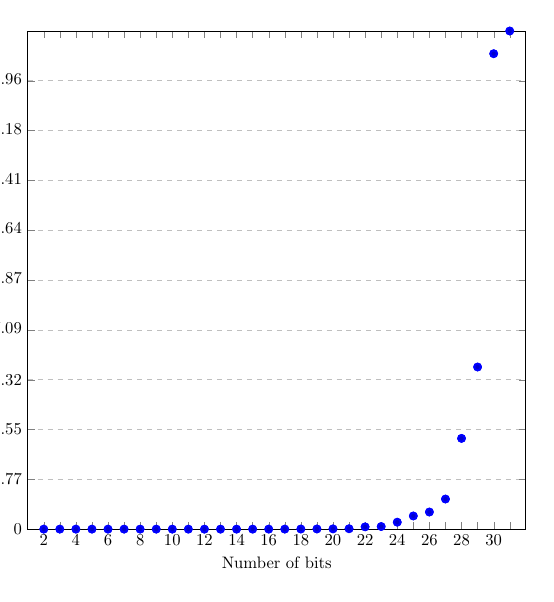
\begin{tikzpicture}[scale=0.6, trim axis left, trim axis right]
\begin{axis}[
    width=1\textwidth,
    height=1\textwidth,
    xlabel={Number of bits},
    ylabel={Time taken (s)},
    xmin=1.0, xmax=32.0,
    ymin=2.5e-05, ymax=3317.729958,
    xticklabels={2, , 4, , 6, , 8, , 10, , 12, , 14, , 16, , 18, , 20, , 22, , 24, , 26, , 28, , 30},
    xtick={2, 3, 4, 5, 6, 7, 8, 9, 10, 11, 12, 13, 14, 15, 16, 17, 18, 19, 20, 21, 22, 23, 24, 25, 26, 27, 28, 29, 30, 31},
    ytick={2.5e-05, 331.7730183, 663.5460116, 995.3190049, 1327.0919982, 1658.8649915, 1990.6379848, 2322.4109781, 2654.1839714, 2985.9569647},
    ymajorgrids=true,
    grid style=dashed,
]

\addplot+[
    blue,
    very thick,
    forget plot,
    only marks
    ]
    plot[
    very thick,
    error bars/.cd,
    y dir=plus,
    y explicit
    ]
    table[x=x,y=y,y error expr=\thisrow{y-max}] {
    x    y    y-max
    24	46.343519	0.303535
25	87.671617	0.0
26	114.011857	0.0
27	200.506368	0.0
20	1.7816451	0.0099209
21	2.7334088	0.0124842
22	15.1897874	0.0405596
23	17.2848708	0.0968762
28	604.359222	0.0
29	1079.771318	0.0
3	3.6e-05	1e-06
2	9.92e-05	0.0006538
5	9.65e-05	8.5e-06
4	6.69e-05	1.1e-06
7	0.0002478	2.52e-05
6	0.0001303	1.17e-05
9	0.0008995	1.35e-05
8	0.0003846	5.4e-06
11	0.0022981	4.79e-05
10	0.0016313	8.7e-06
13	0.0202252	0.0139458
12	0.0112163	0.0006427
15	0.0520107	0.0003753
14	0.0293946	0.0005424
17	0.204421	0.02304
16	0.1269137	0.0005663
19	1.1880814	0.0064836
18	0.8096179	0.0320171
31	3317.729958	0.0
30	3166.677136	0.0

    };

\addplot+[
    blue,
    very thick,
    forget plot,
    only marks
    ]
    plot[
    very thick,
    error bars/.cd,
    y dir=plus,
    y explicit
    ]
    table[x=x,y=y,y error expr=\thisrow{y-min}] {
    x    y    y-min
    24	46.343519	-0.204036
25	87.671617	0.0
26	114.011857	0.0
27	200.506368	0.0
20	1.7816451	-0.0146871
21	2.7334088	-0.0110068
22	15.1897874	-0.0581414
23	17.2848708	-0.0764928
28	604.359222	0.0
29	1079.771318	0.0
3	3.6e-05	-1e-06
2	9.92e-05	-7.42e-05
5	9.65e-05	-1.5e-06
4	6.69e-05	-9e-07
7	0.0002478	-2.8e-06
6	0.0001303	-4.3e-06
9	0.0008995	-4.5e-06
8	0.0003846	-1.6e-06
11	0.0022981	-2.11e-05
10	0.0016313	-1.03e-05
13	0.0202252	-0.0031632
12	0.0112163	-0.0001823
15	0.0520107	-0.0005167
14	0.0293946	-0.0003306
17	0.204421	-0.004761
16	0.1269137	-0.0005107
19	1.1880814	-0.0035704
18	0.8096179	-0.0088229
31	3317.729958	0.0
30	3166.677136	0.0

    };

\end{axis}
\end{tikzpicture}
\vspace{-0.3cm}
\caption{Factors between 2 and 31 bits}\label{fig:TrialDivisionGrowingprimesbits}
\end{figure}

